The Implicit Function Theorem (IFT) allows us to predict the impact of sudden demand shocks on the equilibrium paths for drilling and production. Applying the IFT to equation (\ref{Equation:Firms-Problem_Euler-Equation}) (i.e., the Euler equation of the firm's problem) yields
\begin{align}
    % \frac{ \ f_{ik} \ + \ \lambda_{a} \sigma \big( \gamma \ - \ \ln(1 - Pr_{k}) \big) \ }{\rho} \
    % & = \ \left\{ \psi_{i1k} \ + \ \sigma \big( \gamma \ - \ \ln(Pr_{k}) \big) \right\} \ - \ \sigma \big( \gamma \ - \ \ln(1 - Pr_{k}) \big) \\
    % \frac{1}{\rho} \frac{\partial f_{ik}}{\partial p_{k}} \ + \ \frac{\lambda_{a} \sigma}{\rho (1 - Pr_{k})} \frac{\partial Pr_{k}}{\partial p_{k}} \
    % & = \ \frac{\partial \psi_{i1k}}{\partial p_{k}} \ - \ \frac{\sigma}{Pr_{k}} \frac{\partial Pr_{k}}{\partial p_{k}} \ - \ \frac{\sigma}{1 - Pr_{k}} \frac{\partial Pr_{k}}{\partial p_{k}} \\
    % \left( \frac{\lambda_{a} \sigma}{\rho (1 - Pr_{k})} \ + \ \frac{\sigma}{Pr_{k}} \ + \ \frac{\sigma}{1 - Pr_{k}} \right) \frac{\partial Pr_{k}}{\partial p_{k}} \
    % & = \ -\frac{1}{\rho} \frac{\partial f_{ik}}{\partial p_{k}} \ + \ \frac{\partial \psi_{i1k}}{\partial p_{k}} \\
%    \frac{\partial Pr_{k}}{\partial p_{k}} \
%    & = \ \left\{ \frac{\rho Pr_{k} (1 - Pr_{k})}{\sigma (\lambda_{a} Pr_{k} + \rho)} \right\} \left( \frac{\partial \psi_{i1k}}{\partial p_{k}} \ - \ \frac{1}{\rho} \frac{\partial f_{ik}}{\partial p_{k}} \right).
    \frac{\partial Pr_{k}}{\partial p_{k}} \
    & = \ \left\{ \frac{\rho Pr_{k} (1 - Pr_{k})}{\sigma (\lambda_{a} Pr_{k} + \rho)} \right\} \frac{\partial \psi_{i1k}}{\partial p_{k}}.
\label{Equation:Equilibrium-Paths_Applying-IFT}
\end{align}
This resulting equation suggests that an unexpected positive price shock will lead to a higher drilling rate. The equation also shows that drilling is more responsive to prices when the relative importance of cost shocks, which is captured by the magnitude of $\sigma$, is small. 
\afterpage{
    \begin{figure}[t!]
        \centering
        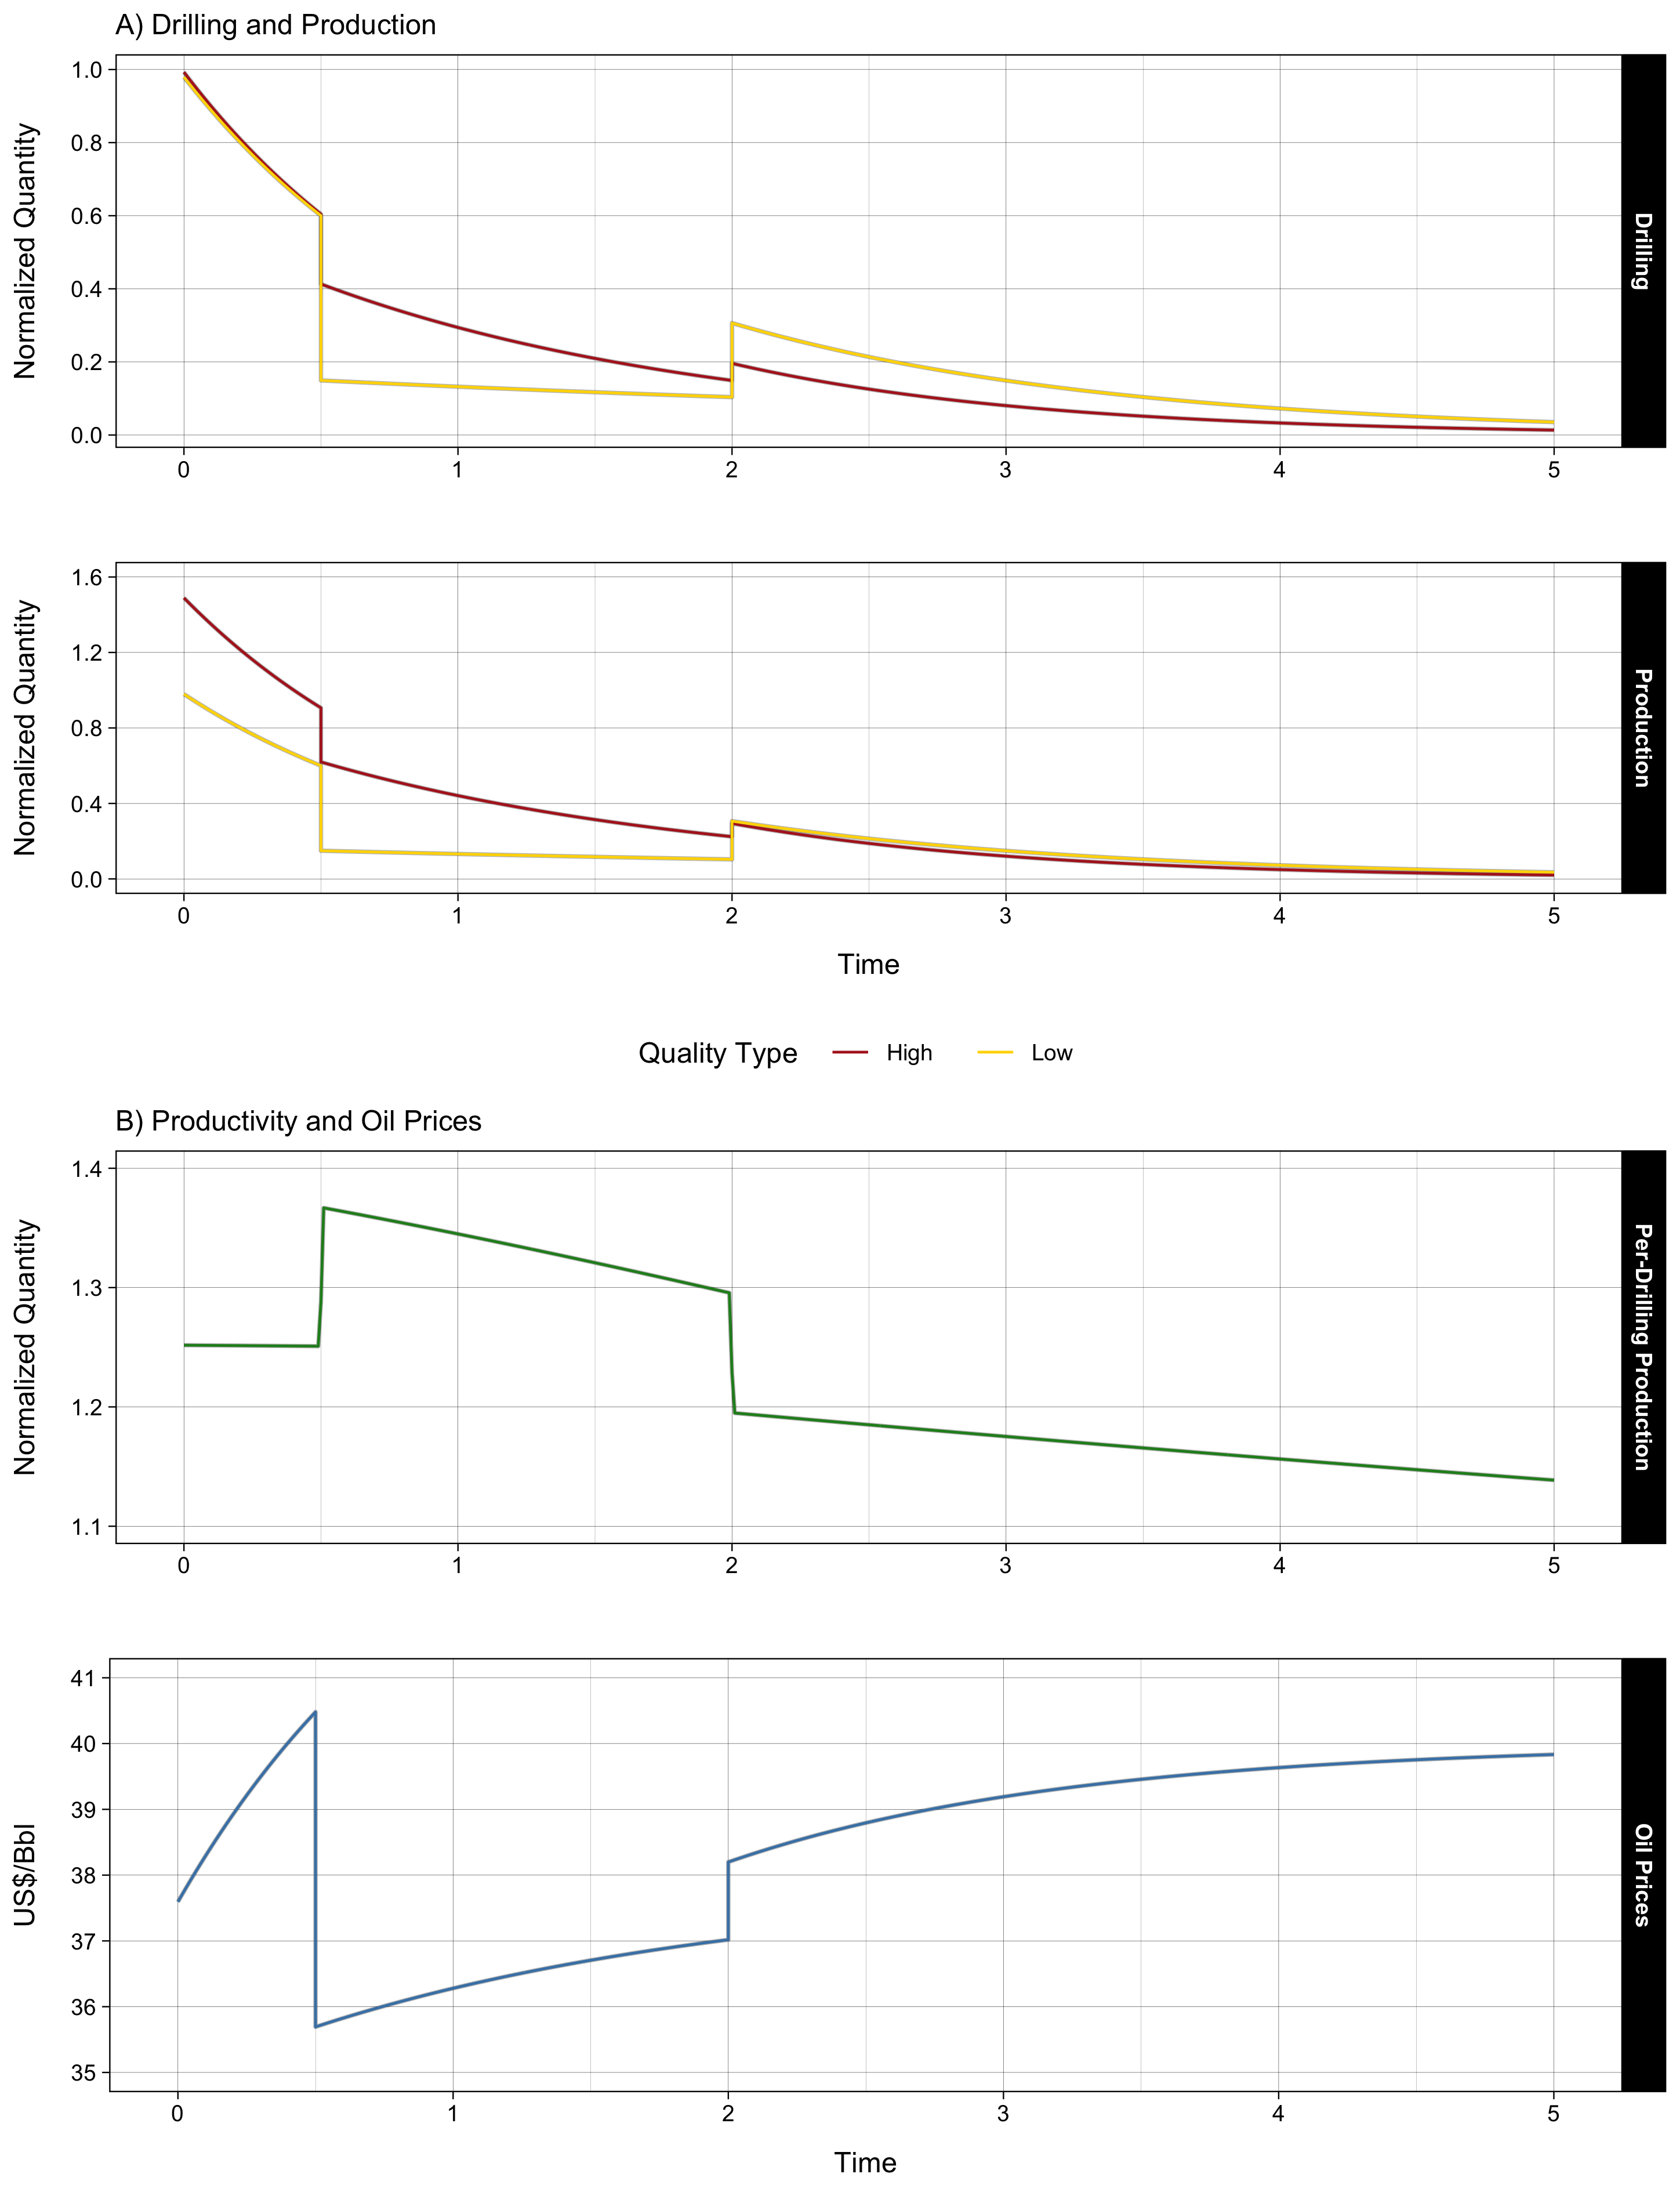
\includegraphics[scale = 0.11]{04_Chapter-3/00A_Figures/Figure_Impact-of-Demand-Shocks-on-Drilling-of-Well-Sites-with-Heterogeneous-Quality}
        \caption{Heterogeneous Impacts of Unexpected Demand Shocks on Drilling and Production}
        \caption*{
            {\small
            \textit{Note}: 
            This figure shows how the firm's drilling activity at well sites of heterogeneous quality responds to unexpected demand shocks. As shown in the first panel, the drilling probability of low-quality well sites shows a higher sensitivity to the first negative demand shock. Although the drilling probability of low-quality well locations more sensitively responds to the second positive demand shock, the probability is still lower than that of high-quality well sites. The second panel demonstrates the time paths of drilling, corresponding to the drilling probabilities. The third panel illustrates the impacts of the demand shocks on oil extraction productivity. Clearly, the first negative shock discontinuously increases per-drilling oil production due to the high sensitivity of low-quality location drilling. To the second positive demand shock, the per-drilling production showed the opposite reaction. For this simulation, we assume that a dispersion parameter of $\sigma = 1$, a discount rate of $\rho = 0.05$, an initial number of well sites of $R_{0}^{g} = 1$, additional well sites of $E^{g} = 0$, where $g \in \{ L, H \}$. Also, we assume that a flow payoff function of $f(p_{k}) = 1$ and that a choice-specific instantaneous payoff function of $\psi_{iak} (p_{k}) = 1.5p_{k} - 2$ for high-quality sites.  
        }}
        \label{Figure:Heterogeneous-Impacts-of-Unexpected-Price-Shocks-on-Equilibrium-Paths}
    \end{figure}
}

Figure \ref{Figure:Equilibrium-Paths-under-Unexpected-Demand-Shocks} depicts how the paths of drilling probability, drilling, reserves, and oil price respond to two unanticipated demand shocks. The first negative demand shock causes drilling probability discontinuously decreases. Due to the reduction in drilling probability, drilling demonstrates a discontinuous decrease too. Moreover, the negative demand shock also reduces the depletion rate of the remaining well locations. As shown in the last panel in the figure, the oil price jumps down on impact after the negative demand shock, then gradually rises.\footnote{Drilling, and thus production, rapidly diminishes for a while after $t = 0$. Then, its rate of change gradually decreases, and drilling eventually converges to a lower bound. In other words, the time path of drilling has a convex profile. Because equation (\ref{Equation:Firms-Problem_Oil-Prices}) determines the oil price at time $t$, the time path for the endogenous oil price is a concave curve.} The later positive demand shock induces the opposite reactions in the equilibrium paths. 
